\documentclass[a4paper,11pt]{article}
\usepackage[british]{babel}
\usepackage[top=1.5cm,bottom=1.5cm,left=1.5cm,right=1.5cm]{geometry}
\usepackage{graphicx}
\usepackage[hyphens]{url}
\usepackage{paralist}
\usepackage{authblk}
\usepackage{siunitx}
\usepackage[noadjust]{cite}
\usepackage[pdftex,colorlinks=true]{hyperref}


% title
\title{Reproducibility in Research: Systems, Infrastructure, Culture}
%\title{Towards ``Reproducibility-as-a-Service''}
%\title{``Reproducibility-as-a-Service'':\\A Model for Reproducible Computational Research}
%\title{``Can I Implement Your Algorithm?'':\\A Model for Reproducible Research Software}

% names
\author[1]{Tom Crick}
\author[2]{Benjamin A. Hall}
\author[3]{Samin Ishtiaq}
% affiliation
\affil[1]{Department of Computing \& Information Systems, Cardiff
  Metropolitan University, UK}
\affil[2]{MRC Cancer Unit, University of Cambridge, UK}
\affil[3]{Microsoft Research Cambridge, UK}
% emails
\affil[1]{\protect\url{tcrick@cardiffmet.ac.uk}}
\affil[2]{\protect\url{bh418@mrc-cu.cam.ac.uk}}
\affil[3]{\protect\url{samin.ishtiaq@microsoft.com}}

\renewcommand\Authands{ and }
\def\UrlBreaks{\do\/\do-}

\date{ }

\begin{document}
\maketitle

% Keywords:
% reproducible research; cyberinfrastructure; scientific workflows; computational
% science; open science; data sharing; code sharing; best practices


\begin{abstract}
The reproduction and replication of novel results has become a major
issue for a number of scientific disciplines. In computer science and
related computational disciplines such as systems biology, the issues
closely revolve around the ability to implement novel algorithms and
models. Taking an approach from the literature and applying it to a
new codebase frequently requires local knowledge missing from the
published manuscripts and project websites. Alongside this issue,
benchmarking, and the development of fair --- and publicly available
--- benchmark sets present another barrier.

In this paper, we outline several suggestions to address these issues,
driven by specific examples from a range of scientific domains.
Finally, based on these suggestions, we propose a new open automated
platform for scientific software development which effectively
abstracts specific dependencies from the individual researcher and
their workstation, allowing easy sharing and reproduction of
results. This new cyberinfrastructure for computational science offers
the potential to incentivise a culture change and drive the adoption
of new techniques to improve the efficiency of scientific exploration.
\end{abstract}

\section{Introduction}

Marc Andreessen (co-author of Mosaic, the first widely used Web
browser) boldly stated in 2011 that ``{\emph{software is eating the
world}}''~\cite{andreessen:2011}. It is true: we clearly live in a
computational world, with our everyday communications, entertainment,
shopping, banking, transportation, national security, etc, all heavily
dependent on (or replaced by) software.

This is particularly true for science and engineering. A 2012 report
by the Royal Society stated that computational techniques have
``{\emph{moved on from assisting scientists in doing science, to
transforming both how science is done and what science is
done}}''~\cite{rssaaoe:2012}. Many of the examples discussed in this
paper take advantage of a fundamental advantage of computer science
and more broadly, computational science: the unique ability to share
the raw outputs of their work as software and datafiles. New
experiments, simulations, models, benchmarks, even proofs cannot be
done without software. And this software does not consist of simple
hack-together, use-once, throw-away scripts; scientific software
repositories contain thousands, perhaps millions, of lines of code and
they increasingly need to be actively supported and maintained. More
importantly, with reproducibility being a fundamental tenet of
science, they need to be re-useable.

However, if we closely analyse the scientific literature related to
software tools it often does not appear to be adhering to these
rules~\cite{nature:2011}. How many of them are reproducible? How many
explain their experimental methodologies, in particular the basis for
their benchmarking? In particular, can we (re)build the
code~\cite{collberg-et-al:2014}? We, the authors, are perhaps as
guilty as anyone in the past, where we have published
papers~\cite{crick-et-al:2009a,Berdine2011SLAyer} with benchmarks and
promises of code to be released in the near future.

There are numerous reasons why the wider scientific community is in
this state. We are currently undergoing significant changes to
academic dissemination and publication, especially the open access
movement, with new models being
proposed~\cite{deroure:2010,stodden-et-al:2013,fursin+dubach:2014}. Journals
such as Nature, PLoS Computational Biology and Bioinformatics
explicitly require that source code and data is made available online
under some form of open source license. While these initiative are
great, they are often optional, seem piecemeal, and do little to
enable verification or validation of scientific results at a later
stage. Even within the same field, there are different ideas of what
defines reproducibility.

Nevertheless, the reproduction and replication of reported scientific
results has become a widely discussed topic within the scientific
community~\cite{barnes:2010,morin-et-al:2012,joppa-et-al:2013}.
Whilst the retraction of several studies has drawn the focus of many
commentators, automated systems, which allow easy reproduction of
results, offer the potential to improve the efficiency of scientific
exploration and drive the adoption of new techniques. But just
publishing (linked) scientific data is not enough to ensure the
required reusability~\cite{bechhofer-et-al:2013}. There exists a wider
socio-cultural problem that pervades the scientific community, with
estimates that as much as 50\% of published studies, even those in
top-tier academic journals, cannot be repeated with the same
conclusions by an industrial lab~\cite{osherovich:2011}. There are
numerous non-technical impediments to making software maintainable and
re-useable. The pressure to ``make the discovery'' and publish quickly
disincentivises careful software curation. Releasing code prematurely
is often seen to give your competitors an advantage, but we should be
shining light into these ``black boxes''~\cite{morin-et-al:2012}. In
essence: better software, better research~\cite{goble:2014}.

Nevertheless, there is promising existing work in this
area~\cite{sim-et-al:2003,chirigati-et-al:2013,stodden+miguez:2014,stodden-et-al:2015},
as well as a number of manifestos for reproducible research and
community initiatives, such as the Recomputation
Manifesto~\cite{gent:2013}\footnote{\url{http://www.recomputation.org/}}
and
cTuning~\cite{fursin-et-al:2014}\footnote{\url{http://ctuning.org/}},
along with curated recommendations on where to publish research
software\footnote{\url{http://www.software.ac.uk/resources/guides/which-journals-should-i-publish-my-software}}.

However, things can, should and need to be much better. Building upon
previous work~\cite{crick-et-al_wssspe2}, we present a call to action,
along with a set of recommendations which we hope will lead to better,
more sustainable, more re-useable software, to move towards an
imagined future practice and usage of scientific software
development. The basis for many of these recommendations is predicated
on the fundamental scientific tenets of openness and sharing.

\section{We Need to Talk About Reproducibility}

% Recommendation I
\subsection{{\emph{Can I Implement Your Algorithm?}}}

Reproducibility is a fundamental tenet of
good science. Yet many descriptions of algorithms are too high-level,
too obscure, too poorly-defined to allow an easy re-implementation by
a third party. A step in the algorithm might say: ``{\emph{We pick an
element from the frontier set}}'' but which element do you pick? Will
the first one do?  Why will any element suffice? Sometimes the author
would like to give more implementation detail but is constrained by
the paper page limit. Sometimes the authors' description in-lines
other algorithms or data structures that perhaps only that author is
familiar with.\\

\noindent {\textbf{Recommendation {\textrm{I}}:}} We recommend here
that a paper must describe the algorithm in such a way that it is
implementable by any reader of that algorithm. This is subjective, of
course. Therefore, we also recommend that relevant scientific
conferences have a special track for papers that re-implement past
papers' algorithms, techniques or tools, as well as incentives to
support sharing of computational artefacts; reproducibility should not
just be discussed at conference and workshops convened explicitly for
that purpose (for example, a number of high-profile computer science
conferences now explicitly acknowledge the importance of
reproducibility, promoting community-driven reviewing and
validation\footnote{\url{http://ctuning.org/cm/wiki/index.php?title=Reproducibility}};
we have recently proposed a new reproducibility model for the
computer-aided formal analysis and verification research
community~\cite{crick-et-al-cav}).


% Recommendation II
\subsection{{\emph{Set The Code Free}}}

There can be no better proof that your algorithm works, than if you
provide the source code of an implementation. Software development is
hard, but sharing and re-using code is relatively easy.

Many years ago, Richard Stallman (founder of the GNU Project and Free
Software Foundation) postulated that all code would be
free~\cite{rms:2010} and we would make our money by consulting on the
code.  As it turns out, this is now the case for a significant
part of the computing industry. There are, of course, hard commercial
pressures for keeping code closed-source. Even in the scientific
domain, scientists and their collaborators may wish to hold onto their
code as a competitive advantage, especially if there exists larger
competitors who could use the available code to ``reverse scoop'' the
inventors, charging into a promising new research area opened by the
inventors.

Closed source is one thing. Licenses that deny the user from viewing,
modifying, or sharing the source are another thing. There are,
however, even licences on widely adopted tools like
GAUSSIAN~\cite{Giles2004} that prohibit even analysing software
performance and behaviour. For example, a wide variety of licenses
exist for molecular dynamics software, with different degrees of
openness (GROMACS uses the GNU Lesser General Public License
(LGPL)~\cite{Hess2008}, CHARMM and Desmond are Academic/Commercial
software licences~\cite{Brooks2009,Bowers2006}, Amber and NAMD are
custom open-like licences). Z3 is an example from the verification
area: the code itself is not open source, but the MSR-LA license that
allows the source code to be read, copied, forked for academic use,
provides researchers in the field much more than
before~\cite{deMoura2012Z3open}.\\
 
\noindent {\textbf{Recommendation {\textrm{II}}:}} There is little
doubt that, if science wants to be open and free, then the code that
underlies it too needs to be open and free. Code that is available for
browsing, modifying, and forking facilitates testing and comparison,
and promotes competition. We recommend that code be published under an
appropriate open source license~\cite{osl}; while we defer legal
discussion of the specifics of any particular licences, BSD and Apache are good,
flexible ones.\\
% IANAL...

\noindent Ultimately: set the code free and make it available on a public
repository such as GitHub, where it is easy to share and fork -- it is
good enough~\cite{barnes:2010}.

% Recommendation III
\subsection{{\emph{Be A Better Person}}}

If you have the appropriate skills and the experience, you can always
create better software. We have seen the emergence of successful
initiatives, such as the Software Sustainability
Institute\footnote{\url{http://www.software.ac.uk/}}, Software
Carpentry\footnote{\url{http://software-carpentry.org/}} and the UK
Community of Research Software
Engineers\footnote{\url{http://www.rse.ac.uk}}, in cultivating
world-class research through software, developing software skills and
raising the profile of research software engineers.

Many scientists will not have had any formal, or even informal,
training in scientific software development. Even basic training in
software engineering concepts like version control (git, mercurial),
unit testing (tests written to exercise the smallest testable parts of
a system, like a function exported from a module), regression testing
(a test framework that ensures that previous results are maintained
over the changes in the source code), build tools (Make, scons), etc,
can help improve the quality of the software written
enormously~\cite{wilson2006}.  Interestingly, many of these concepts
are taught to computer science undergraduates, but it could be argued
that they are taught at the wrong time of their careers, without the
experience of complex,
long-running projects.\\
%\footnote{\url{http://philipwfowler.wordpress.com/2013/12/19/the-oxford-software-carpentry-boot-camp-one-year-on/}}.

\noindent {\textbf{Recommendation {\textrm{III}}:}} Software
development skills should be regarded as fundamental literacies for
scientists and engineers: we recommend that basic programming and
computational skills are taught as core at undergraduate and
postgraduate level.

% Recommendation IV
\subsection{{\emph{The Lingua Franca of Computational Science}}}

There is no other scientific or technical field where its participants
can just make up a non-principled artefact like a programming language
so easily. In a way, it shows how much of a ``commons'' computer
science has become, that anyone can create a new programming language,
API, framework or compiler. This clearly has its advantages and
disadvantages.

High-level languages are generally more readable than their
competitors. The ``density'' of a program is often seen to be a good
thing, but it is not always the case that a shorter Haskell program
(for example) is easier to maintain than a longer Python/C++
one. Nevertheless, what is important is the readability of the code
itself. A good example here is from the world of automatic theorem
proving: the SSReflect language is much more readable than the
original, standard Coq language~\cite{GonthierZND13}. SSReflect uses
mathematicians' vernacular for script commands, allows reproducibility
of automatic proof-checking because parameters are named rather than
numbered.  Even though these proof scripts are really only ever going
to be run by a machine, they seek to maintain the basic mathematical
idea that a proof should be readable by another mathematician.

High-level programming languages impose constraints like types: that
you can never add a number and a string is the most basic example, but
ML's functors provide principled ways of plugging in components with
their implementations completely hidden. Aggressive type checking
avoids a subset of bugs which can arise due to incorrectly written
functions e.g. well publicised problems with a NASA Mars
orbiter\footnote{\url{http://www.cnn.com/TECH/space/9909/30/mars.metric.02/}}.
A further example is a pressure coupling
bug\footnote{\url{http://redmine.gromacs.org/issues/14}} in
GROMACS~\cite{Hess2008}, which arose due to the inappropriate swapping
of a pressure term with a stress tensor.  A further extension of
types, a concept called units of measure that is implemented in
languages such as F\#, can deal with these kinds of bugs at compile
time. Similarly, problems found using in-house software for
crystallography led to the retraction of five
papers~\cite{Miller2006}, due to a bug which inverted the phases.\\

\noindent {\textbf{Recommendation {\textrm{IV}}:}} The use of a
principled, high-level, typed programming language in which to write
your software helps hugely with the maintainability, robustness and
openness of the software produced. Use Typescript or Flow rather than
plain old Javascript; use Hack rather than PHP. 

% Recommendation V
\subsection{{\emph{Lineage (or: ``Standing On The Shoulders Of Giants'')}}}

Research software is not just software -- it is the instantiation of
novel algorithms and data structures (or at least novel applications
of data structures). Thus, lineage is important:\\

\noindent {\textbf{Recommendation {\textrm{V}}:}} Code should always
include links to papers publishing key algorithms and the code should
include explicit relationships to other projects on the repository
(i.e. {\emph{Project B}} was branched from {\emph{Project A}}). This
ensure that both the researchers and software developers working
upstream of the current project are properly credited, encouraging
future sharing and development. Remember, the people who did the
research are not necessarily the same people as the developers and
maintainers of the software, so it is important to reward both
appropriately with citations (a good way of doing this is the use of
CITATION
files\footnote{\url{http://blog.rtwilson.com/encouraging-citation-of-software-introducing-citation-files/}}).

% Recommendation VI
\subsection{{\emph{YMMV}}}

\begin{figure}[!ht]
\centering
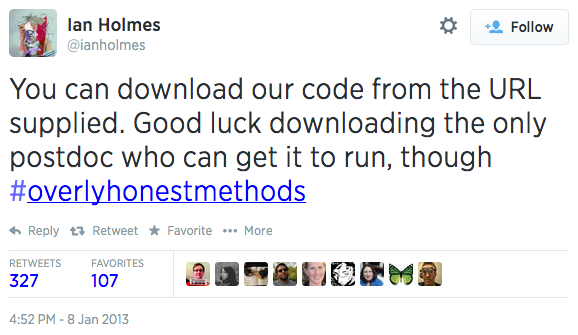
\includegraphics[width=0.8\textwidth]{images/overlyhonesttweet.png}
\caption{{\texttt{\#overlyhonestmethods}} on Twitter\newline [source: \url{https://twitter.com/ianholmes/status/288689712636493824}]}
\label{fig:overlyhonestmethod} 
\end{figure}

The tweet in Figure~\ref{fig:overlyhonestmethod} is sad but worryingly
true, highlighting the perils of reproducible
research\footnote{\url{http://www.phdcomics.com/comics.php?f=1689}}. Often,
the tool that the paper describes does not exist for download. Or runs
only on one particular bespoke platform. Or might run for the author,
for a while, but will `bit-rot' so quickly that even the author cannot
compile it in a couple of month's time.\\

\noindent {\textbf{Recommendation {\textrm{VI}}:}} Providing the
source code of the tool helps, of course. But you must also provide
details of precisely \emph{how} you built and wrote the software. For
example:

\begin{itemize}
\item you should provide the compiler and build toolchain; 
\item you should provide build tools (e.g. Makefiles/Ant/etc) and
  comprehensive build instructions; 
\item you should list or link to all non-standard packages and libraries that you use; 
\item you should note the specifics of the hardware and OS used. 
\end{itemize}

This may appear to be significant extra overhead for researchers, but
GitHub APIs, continuous integration servers, virtual machines and
cloud environments can make it easier; see
Section~\ref{sec:conclusion} for more on this.


% Recommendation VII
\subsection{{\emph{Data Representations and Formats}}}

We often do not, and should not, care how things are stored on disk,
what their precise representations are. But a common, constrained,
standard representation is good for passing tests or models around
between different tools. A properly described representation, like the
SMT-LIB format\footnote{\url{http://smt-lib.org}} for Satisfiability
Modulo Theory (SMT) solvers, where both the syntax and semantics are
well understood, hugely aids developing tools, techniques and
benchmarks.

Another example, from biology, is that of the standard representation
of qualitative networks and Boolean
networks~\cite{Kauffman1969,Schaub2007}.  These networks can be
expressed in SMV format, but this would mean that standard
qualitative/Boolean network behaviours have to be hard-coded for each
variable, introducing the possibility for errors. In the
BioModelAnalyzer tool~\cite{Benque2012}, the XML contains \emph{only}
the modifiable parameters limiting the possibility for error.\\

\noindent {\textbf{Recommendation {\textrm{VII}}:}} Avoid creating
new representations when common formats already exist. Use existing
extensible internationally standardised representations and formats to
facilitate sharing and re-use.

% Recommendation VIII
\subsection{{\emph{World Records}}}

The benchmarks the tool describes are fashioned only for this instance
of this time. They might claim to be from the Windows device driver
set, but the reality is that they are stripped down versions of the
originals. Stripped down so much as to be useless to anyone but the
author vs. the referee. It is worse than that really: enough
benchmarks are included to beat other tools. The comparisons are never
fair (neither are other peoples' comparisons against your tool). If
every paper has to be novel, then every benchmark, too, will be novel;
there is no monotonic, historical truth in new, synthetically-crafted
benchmarks. It is as if, in order to beat Usain Bolt's
\num{100}\si{\metre} world record time, you make him wear boots on a
muddy icy track, weighing him down with \num{50}\si{\kilogram} of
excess weight. Given this setup, you could surely hope to beat his
\num{9.58}\si{\second} time on a shorter length track.\\

\noindent {\textbf{Recommendation {\textrm{VIII}}:}} Benchmarks should
be public. They should allow anyone to contribute, implying that the
tests are in a standard format. Further, these benchmarks must be
heavily curated. Every test/assertion should be justified. Papers
should be penalised if they do not use these public benchmarks. While
there are some domains in which it may not be immediately possible to
share full benchmarks sets, this should be the exception (with
justification) rather than the norm.\\

A good example of some of these points is the RCSB Protein Data
Bank\footnote{\url{http://www.pdb.org}} and Systems Biology Markup
Language~\cite{Chaouiya2013}. The software ones we know of,
the SMT
Competition\footnote{\url{http://smtcomp.sourceforge.net/2014/}},
SV-COMP\footnote{\url{http://sv-comp.sosy-lab.org/2015/}} and
Termination Problems Data
Base\footnote{\url{http://termination-portal.org/wiki/TPDB}} are on
that journey. Such repositories would allow the tests to be taken and
easily analysed by any competitor tool.

% Recommendation IX
\subsection{{\emph{Test It To See}}}

Some models may be chaotic and influenced by floating-point errors
(e.g. molecular dynamics), further frustrating testing. For example:
Sidekick is an automated tool for building molecular models and
performing simulations~\cite{Hall2014Sidekick}. Each system is
simulated from an different initial random seed, and under most
circumstances this is the only difference expected between
replicas. However, on a mixed cluster with both AMD and Intel
microprocessors on the nodes, the difference in architecture was found
to alter the number of water molecules added to each system by
one. This meant that the same simulation performed on different
architectures would diverge. Similarly, in a different simulation
engine, different neighbour searching strategies gave divergent
simulations due to the differing order in which forces were summed.

A further example is the handling of pseudo-random number generation
in Avida~\cite{ofria+wilke:2004}, an open source scientific software
platform for conducting and analysing experiments with
self-replicating and evolving computer programs. While it may
initially appear attractive to develop bespoke random number
generators within a system for consistency or performance across
platforms, this invariably adds complexity to your system and may
inhibit sharing and reproducibility.\\

\noindent {\textbf{Recommendation {\textrm{IX}}:}} Despite these
challenges to testing, unshared code is ultimately untestable.
Testing new complex scientific software is difficult -- until the
software is complete, unit tests may not be available. You should aim
to re-use modules or repos (git submodules) from publicly-shared
code. An implication of Linus's Law (``given enough eyeballs, all bugs
are shallow'') might be that shared code is inherently more test-able.


% Recommendation X
\subsection{{\emph{Welcome to Web 2.0}}}

Virtual machines (VMs) in the cloud also make the testing of scaling
properties more simple.  If you have a tool that you claim is more
efficient, you could put together a cluster of slow nodes in the cloud
to demonstrate how well the software scales for parallel calculations.
Cloud computing is cheap, and getting cheaper. Algorithms that used to
require massive HPC resources can now be run cheaply by bidding on the
VM spot market. The Web is a great leveller: use and share workflows
and web services~\cite{crick-et-al:2009b,oabarriaga-et-al:2014}.\\

\noindent {\textbf{Recommendation {\textrm{X}}:}} The Web and the
cloud really do open up a whole new way of working. Even small,
seemingly trivial features like putting up a web interface to your
tool and its tests will allow users who are not able to install
necessary dependencies to explore the running of the tool
\cite{Hall2014}. Ultimately, this can lead to making an ``executable
paper'' appear on the Internet. The interactive {\em Try
F\#}\footnote{\url{http://www.tryfsharp.org/Learn}} and Z3
tutorials\footnote{\url{http://rise4fun.com/Z3/tutorial/guide}} are a
great start that begin to expose what can be done in this area.
% removed: ~\cite{tryFsharp} ~\cite{Z3tutorial}


\section{A Model for Reproducible Research Software}\label{sec:conclusion} 
%\section{Conclusions: A New Model}

Some of the Recommendations above, like ``Be A Better Person'' or
``The Lingua Franca'', are abstract, airy-fairy, pie-in-the-sky
even. However, most of them can be concretely realized by a service
for reproducibility. This service provides a concrete implementation
of free source code (``Set The Code Free'') that depends on other free
source code (``Lineage'') building (``YMMV'', ``Welcome to Web 2.0'')
and running tests contributed in public (``Data Representations'',
``World Records'') in a completely reproducible regime.

The service we describe here can be seen as a specification. We
haven't built it, but many servics like travis-ci or Azure VSTS
provide some of the mechanical parts of it. 

A service for reproducibility is intended to play three important
roles. It should:

\begin{enumerate}
\item Demonstrate that a piece of code can be compiled, run
and behaves as described, without manual intervention from the
developer.
\item Store and link specific artefacts with their linked
publications or other publicly-accessible datasets.
\item Allow new benchmarks to be added, by users other than
the developer, to widen the testing and identify potential bugs.
\end{enumerate}

The whole premise of our previous paper~\cite{crick-et-al_recomp2014}
is that {\emph{algorithms}} (implementations) and {\emph{models}}
(benchmarks) are inextricably linked. Algorithms are designed for
certain types of models; models, though created to mimic some physical
reality, also serve to stress the current known algorithms. An
integrated autonomous open cloud-based service can make this link explicit.

By developing a cloud-based, centralised service, which performs
automated code compilation, testing and benchmarking (with associated
auditing), we will link together published implementations of
algorithms and input models. This will allow the prototype to link
together software and data repositories, toolchains, workflows and
outputs, providing a seamless automated infrastructure for the
verification and validation of scientific models and in particular,
performance benchmarks. The program of work will lead the cultural
shift in both the short and long-term to move to a world in which
computational reproducibility helps researchers achieve their goals,
rather than being perceived as an overhead.

A system as described here has several up-front benefits: it links
research papers more closely to their outputs, making external
validation easier and allows interested users to explore unaddressed
sets of models. Critically, it helps researchers across computational
science to be more productive, rather than reproducibility being an
overhead on their day-to-day work. In the same way that tools such as
GitHub make collaborating easier while simultaneously allowing
effortless sharing, we envisage our system being similarly usable for
sharing and testing algorithms, software, models and benchmarks
online.

Suppose you have come up with a better algorithm to deal with some
standard problem.  You write up the paper on the algorithm, and you
also push an implementation of your algorithm to the our cloud
environment's section on this standard problem. The effect of pushing
your implementation is to register your program as a possible
competitor in this standard problem competition. There are several
dozen widely-agreed tests on this problem already on our cloud
environment's database. Maybe, after some negotiation due to your
novel approach to this standard problem, you add some of your own
tests to the database too.

Pushing your code activates the environment's continuous integration
system.  The cloud pulls in all the dependencies your code needs, on
the platforms you specify, and runs all the benchmarks. This happens
every time you push. It also happens every time one of your
dependencies (a library, a firmware upgrade for your platform, a new
API) changes too. This system (presented in Figure~\ref{fig:workflow})
would integrate with publicly available source code repositories,
automates the build, testing and benchmarking of algorithms and
benchmarks. It would allow testing models against competing
algorithms, and the addition of new models to the test suite (either
manually or from existing online repositories).

\begin{figure}[!ht]
\centering
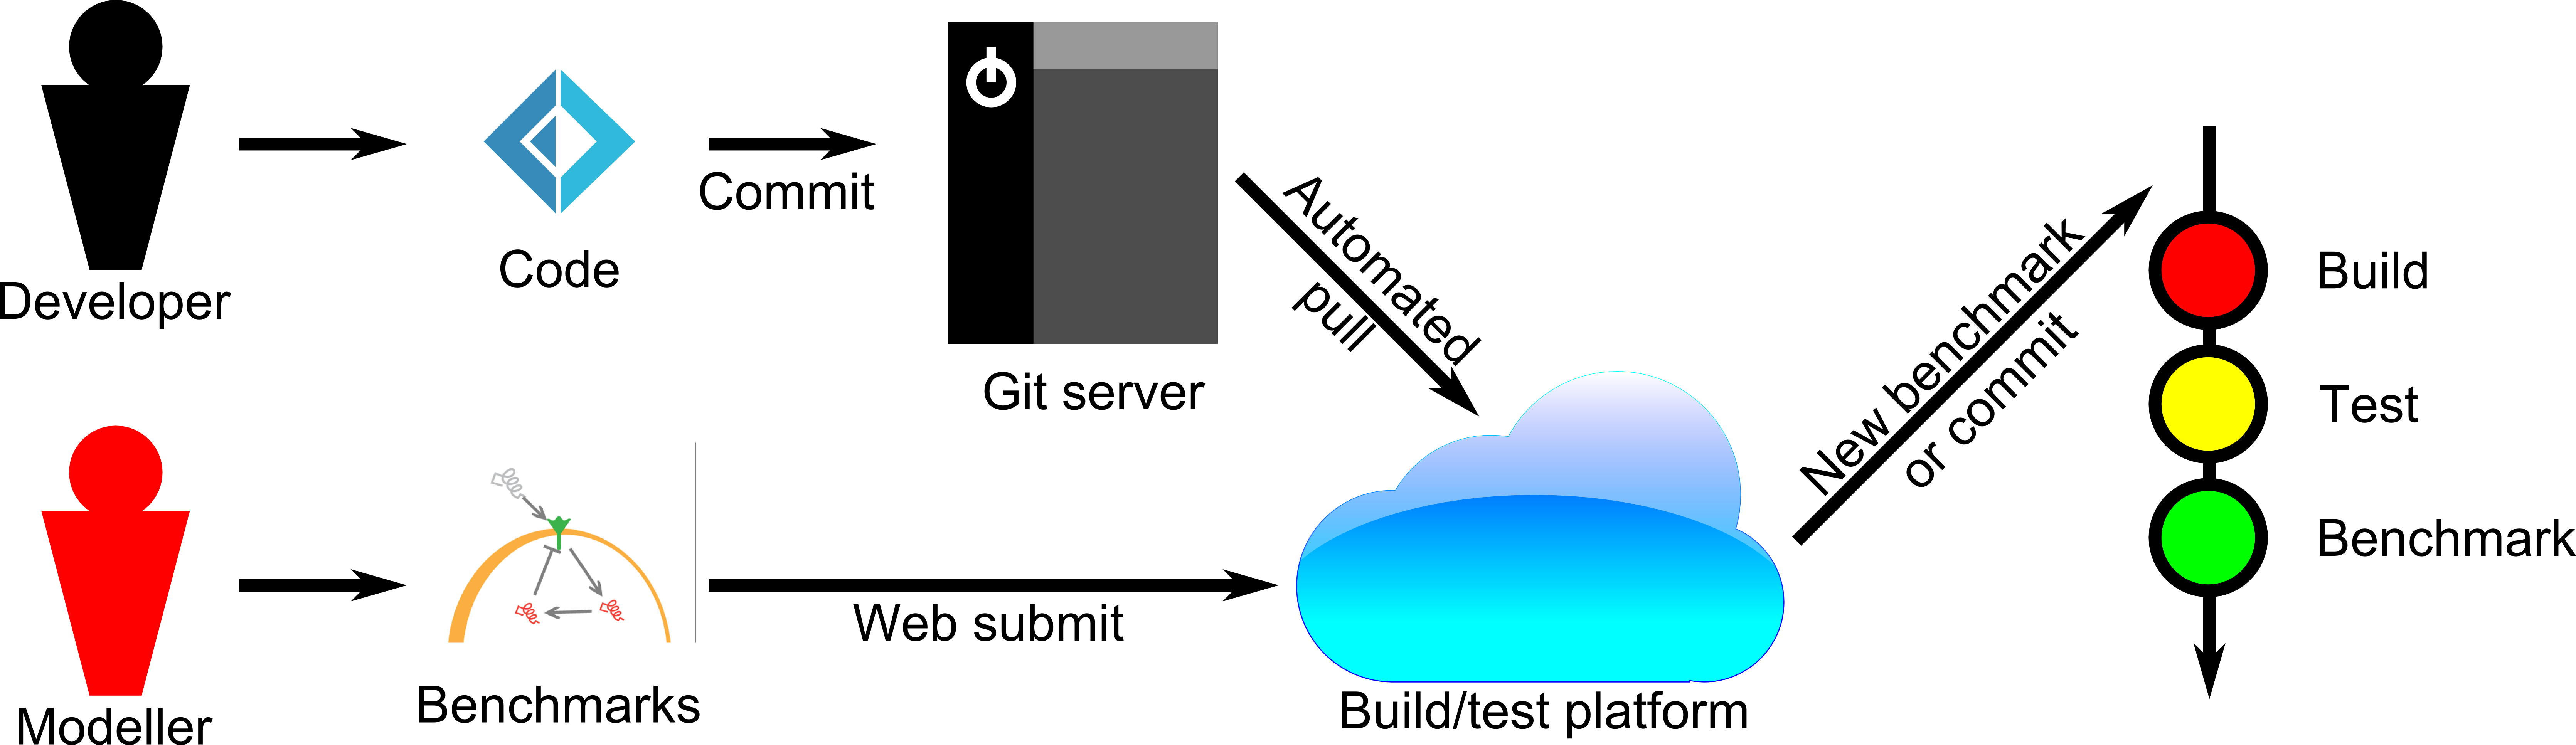
\includegraphics[width=0.9\columnwidth]{images/workflow.png}
\caption{Proposed reproducibility service workflow}
\label{fig:workflow} 
\end{figure}

If we are truly serious about addressing the systemic socio-technical
issues in scientific disciplines that are underpinned by leveraging
software and computational techniques, then the proposal above would
bring together almost all of the points we have discussed in this
paper to provide an open research infrastructure for all. There are
already several web services that already aim to do many of these
things (for example, a repository for disseminating the computational
models associated with publications in the social and life
sciences~\cite{rollins-et-al:2014}), so a service that can integrate
most if not all of these features is possible. Such a service would
then allow algorithms and models to evolve together, and be
reproducible from the outset. Something more complete, and stamped
with the authority of the major domain
conferences/journals/professional societies, would mean that your code
would never `bit-rot', and no one would have problems reproducing the
implementation of your published algorithm.


\section{Next Steps}

Following the proposal of such a system, the question becomes:
{\emph{how do we encourage widespread uptake, or even
standardisation?}}  Such a service would appear to be non-trivial,
given the large numbers of tools and workflows that could potentially
require to be supported by the service. Furthermore, after such a
service has been implemented, how do we ensure it is \emph{useful} and
\emph{usable} for researchers.

The benefits to the wider computational research community from a
cultural change to favour reproducibility are clear and as such we
should aim through software cyberinfrastructure and sharable,
community curated research workflows to mitigate these
costs. Furthermore, we can reasonably expect the distinct needs of
specific research communities to evolve over time, and initial
implementations of the platform may require refinement in response to
user feedback (supporting the critical cultural change by improving
the efficiency of researchers). As such, if the wider research
community is to move to requiring reproducibility, it seems most
reasonable that this is staggered over a number of years to allow for
both of these elements to develop, until eventually all researchers
are required to use the service.

The key question for different research communities then becomes:
{\emph{how to initialise this change?}} Such a requirement creates a
set of new costs to researchers, both in terms of time spent ensuring
that their tools work on the centralised system (in addition to their
local implementation), but also potentially in terms of equipment (in
terms of running the system). Such costs may be easier to bear for
some groups compared to others, especially those with large research
groups who can more easily distribute the tasks, and it is important
that the service does not present a barrier to early career
researchers and those with efficient budgets (this type of cost
analysis is not unique to reproducibility efforts -- it has been
estimated that a shift to becoming exclusively open access for a
journal may lead to a ten-fold increase in computer science
publication costs~\cite{vardi-cacm-2014}).

Nevertheless, this proposed new cyberinfrastructure could have a
profound impact on the way that computational science is performed,
repositioning the role of models, algorithms and benchmarks and
accelerating the research cycle, perhaps truly enabling a ``fourth
paradigm'' of data intensive scientific discovery~\cite{hey:2009}. But
ultimately, an open discussion and understanding of what
reproducibility means for the wider computational science research
community is important: we all need to explicitly state that this is
worthwhile and address it, or don't bother doing it at all.


% BibTeX
\bibliographystyle{ieeetr}
\bibliography{jors2015}

\end{document}
